% !TeX spellcheck = en_US
\documentclass[11pt,a4paper,titlepage]{article}
\usepackage[margin=1.25in]{geometry}
\usepackage{blindtext}
\usepackage{enumitem}
\usepackage{xcolor}
\usepackage{hyperref}
\usepackage{graphicx}
\usepackage{caption}
\usepackage{float}
\usepackage[htt]{hyphenat}
\usepackage{amsmath}
\usepackage{subcaption}

\title{\textsc{STAD68 Final Report}\\ Comparison of Random Forests and Support Vector Machines (SVM)}
\author{Guan Yu Chen\\ 1001591967}
\date{Due: December 3, 2018}
\usepackage{fancyhdr}

\pagestyle{fancy}
\fancyhf{}
\lhead{STAD68}
\chead{Report: Comparison of Random Forest and SVM}
\rhead{Guan Yu Chen}
\rfoot{Page \thepage}

\begin{document}
	\maketitle
	\section{Introduction}
	There are lots of machine learning algorithms to use on certain datasets and the decision might be difficult on which one that has the better performance and accuracy. Specifically, this report aims to compare\footnote{since there is some randomness in the initial settings of the algorithms, the seed used is 123} the accuracy and performance of Random Forest and Support Vector Machine (SVM). The dataset that will be used for this comparison is a wine dataset. 
	
	Red and white wine are enjoyed by many around the world but some are tastes better than others. The goal is to analyze different quality red wine, in particular the Portuguese "Vinho Verde". The analysis aims to given a set of characteristics of the wine, is it possible to predict the quality as well as given the quality, is it possible to determine the characteristics. The dataset \footnote{dataset available at \url{https://www.kaggle.com/uciml/red-wine-quality-cortez-et-al-2009}} has a total of 1599 observations, 11 features (not including reponse variable) and 1 response variable (11 wine qualities\footnote{a.k.a 11 classes in total}). Some of the features in the dataset include fixed acidity, citric acid, pH Scale, Alcohol level, residual sugar.
	\section{Setup}
	The data didn't come already split with training and testing set, using \texttt{model.selection.train\_test\_split} the data was split into 70\% training (1119 observations) and 30\% test (480 observations). Of the 70\% of training data, 10\% is used for cross validation. For binary classification the data split by the following rules based the quality of the wine, $q$:
	\begin{enumerate}
		\item If $q\leq 5$, classify as \textit{poor} quality wine
		\item If $q\geq 6$, classify as \textit{good} quality wine
	\end{enumerate}
	The next step was try to classify with 3 classes, similar to binary classification, the classes was divided by the following criteria:
	\begin{enumerate}
		\item If $q\leq 4$, classify as \textit{poor} quality wine
		\item If $q=5$ or $q=6$, classify as \textit{okay} quality wine
		\item If $q\geq 7$, classify as \textit{good} quality wine
	\end{enumerate}
	After, all 11 classes will be used to compare classification results. In order to train the model and choose the best hyperparameter, Out-Of-Bag Error was used. This allows for cross validation to be done in the Random Forest algorithm. 
	\section{Random Forest}
	Random Forest is an ensemble method that can be used for classification and regression. It constructs a multitude of decision trees when training and outputs the class (classification) or mean prediction (regression). Using Random Forests avoids chances of overfitting which single decision trees can do. The implementation of Random Forest is done in Python using built-in libraries. In \texttt{sklearn.ensemble}, which is Sci-Kit Learn library ensemble methods, there is a \texttt{RandomForestClassifier}. To use it, the hyperparameters needs to be adjusted and fit/train the model to the training data. After tuning the hyperparameters, we can test the model on the testing data in order to estimate the true risk. For the metrics, another library was used called \texttt{metrics} from \texttt{sklearn}, this library computes the precision, recall, F1-Score and mean (weighted in some cases) precision. 
	\subsection{Binary Classification}
	First, the Random Forest is trained on the training set with 1000 decision trees, maximum of 3 features considered per split, minimum of 3 samples required to split an internal node, every leaf node have to have a minimum of 2 samples and with Out-Of-Bag Error and splits are determined by calculating entropy. With the above hyperparameters, the Out-Of-Bag Error on training is 0. With this model, the testing data was used to test this model and evaluate its performance. This model also got 0 loss on the testing data. This is expected since this is only a binary classification. 
	\subsection{Classification with 3 Classes}
	The classification for 3 classes was done with the same hyperparameters as the binary case. The Out-Of-Bag precision was slightly less than the binary case at 0.998 (99.4\%). With this model, the testing data was used to test the performance of this model. The weighted average of precision, recall and F1-Score is at 1.00 (100\%), but inspecting the confusion matrix, there is a 0.42\% loss. 
	\begin{figure}[H]
		\centering
		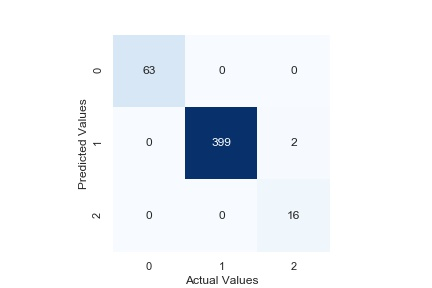
\includegraphics[scale=0.6]{img/threeclass_rf.jpg}
		\caption{Confusion matrix from Random Forest ran on testing data with 3 classes (0 - poor, 1 - okay, 2 - good).}
	\end{figure}
	\noindent The binary and 3 classes models almost had a perfect performance on the test data, the next thing to do is how well it can do on the all classes in the data without simplification. 
	\subsection{Classification with All Classes}
	As mentioned above, the data has a total of 11 classes but most of the wine qualities are between 5 and 8. For the model, we will use the same hyperparameters as the binary and 3 classes classification with Out-Of-Bag Error. From the training, the Out-Of-Bag precision is 82.1\%. This was taken as the lowest case and the hyperparameters were tuned to see if a better Out-Of-Bag precision could be achieved. Adjusting the number of decisions trees used to 1500 and the maximum number of features to be considered for splits to 5, the Out-Of-Bag precision is 0.7\%. Running this model on the test data, the precision is 0.63 (63\%), recall is 0.65  (65\%), F1-Score is 0.63 (63\%) and the loss is 34.58\% calculated from the confusion matrix shown below.
	\begin{figure}[H]
		\centering
		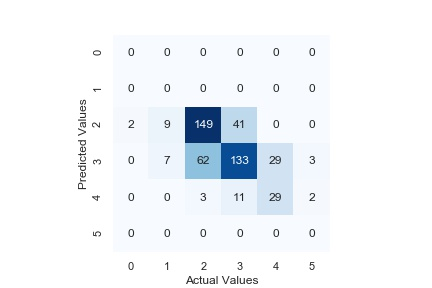
\includegraphics[scale=0.6]{img/allclass_rf.jpg}
		\caption{Confusion matrix from Random Forest ran on testing data with all classes.}
	\end{figure}
	\section{Support Vector Machine (SVM)}
	Support Vector Machine (SVM) is a supervised machine learning algorithm that can be used for either regression or classification, in this case SVM will be used for classification. In this algorithm, each data point is plotted on a n-dimensional space and classification is performed by finding the hyperplane that differentiate between the classes well. In order to adjust the hyperplane, it uses the margin (distance between the hyperplane and the closest points to the hyperplane) to find the best hyperplane to classify the specific dataset. Similar to the implementation of Random Forest, SVM can be done with a built-in library in Python called \texttt{svm} in \texttt{sklearn}. To make a model, the hyperparameters does need to be adjusted and which method to use to determine the hyperplane. The methods include Radial Basis Functions (RBF), polynomial and linear. The metrics will be done using the same library as Random Forest.
	\subsection{Binary Classification}
	In the binary classification case the hyperparameters were left on default; only the kernel function is modified. The model was trained with RBFs and polynomials. The polynomial case has much better performance than the RBFs. With the kernel function as polynomial, performing cross validation with the validation set had 0 loss. Evaluating the model, there was 0 loss on the test data. In contrast with RBFs, cross validation showed a 7.14\% loss. Evaluating the model on the testing data showed the metrics are 93\% precision, 93\% recall, 92\% F1-Score and 7.08\% loss.
	\subsection{Classification with 3 Classes}
	The criteria for the  division of the data into 3 classes was mentioned in the Setup section and similar to the binary case 2 kernel functions was used. First, the kernel function was set to polynomial and a model was trained on the training data. Performing cross validation, it showed the model had a 0 loss on the validation data. Using this model, it was evaluated on the test data and similar to the binary case, the weighted average for precision is 100\%, for recall is 100\% and F1-Score is 100\%. Though the loss in this case is smaller than the binary classification at 0.21\%. Next, another model is trained but with the kernel set to use RBFs. Cross validation showed the model had a 10.7\% loss on the validation data. After cross validation, it is evaluated on the test data. The precision is 90\%, 89\% recall, 87\% F1-Score and 10.83\% loss. The confusion matrix for both polynomial and RBF are shown below:
	\begin{figure}[H]
		\begin{subfigure}{0.4\textwidth}
			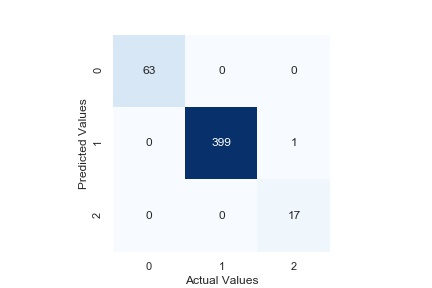
\includegraphics[scale=0.5]{img/threeclass_svmpoly.jpg}
		\end{subfigure}
		\begin{subfigure}{0.4\textwidth}
			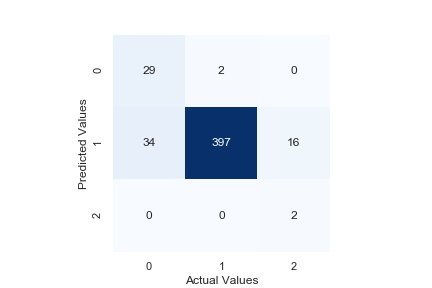
\includegraphics[scale=0.5]{img/threeclass_svmrbf.jpg}
		\end{subfigure}
		\caption{\textbf{Left}: Confusion matrix for SVM with polynomial kernel ran on testing data with 3 classes. \textbf{Right}: Confusion matrix for SVM with RBF kernel ran on testing data with 3 classes.}
	\end{figure}
	\subsection{Classification with All Classes}
	Since there are 11 classes in the dataset, fitting a polynomial on this data will take too long, the SVM was only trained with a RBF kernel. Cross validation showed a 42.86\% loss. This model was then evaluated on the test data, the performance was significantly less than Random Forest, the precision is at 56\%, the recall is 58\%, the F1-Score is at 56\% and the loss is 42.08\% \footnote{if the polynomial kernel didn't take forever to run, it may have performed better}. The confusion matrix is shown below:
	\begin{figure}[H]
		\centering
		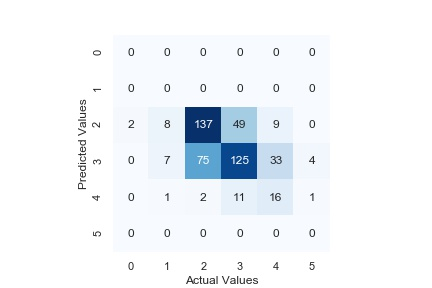
\includegraphics[scale=0.6]{img/allclass_svmrbf.jpg}
		\caption{Confusion matrix from SVM with kernel set to use RBF ran on testing data with all classes.}
	\end{figure}
	\section{Comparison of Random Forest and SVM}
	Given all the results above, Hoeffding's Inequality can be applied to make a comparison. Since a binary classification, classsification with 3 classes and all classes, a comparison can be made in each one. This will be done by computing a 95\% confidence interval for the true risk, defined as:
	\begin{align*}
	\left[L_{S_{\text{test}}}-\sqrt{\frac{log\left(\frac{2}{\delta}\right)}{2m}},L_{S_{\text{test}}}+\sqrt{\frac{log\left(\frac{2}{\delta}\right)}{2m}}\right]
	\end{align*}
	with $m=480$ and $\delta=0.05$.
	\subsection{Binary Classification Comparison}
	Using the results from binary classification, Random Forest had 0 loss and SVM had a 0 loss (taking the polynomial kernel which had the least loss). The 95\% confidence interval for the true risk for Random Forest comes out to be [0, 0.062] and for SVM it is [0, 0.062]. In this case, these Random Forest and SVM are tied with SVM using a polynomial kernel. But with the kernel set to RBF for SVM, the 95\%  confidence interval changed to [0.0088, 0.133], which compared to Random Forest has a higher upper bound, therefore Random Forest performs better than SVM in this case. The confidence intervals are graphed below to better visualize.
	\begin{figure}[H]
		\centering
		\begin{subfigure}{0.4\textwidth}
			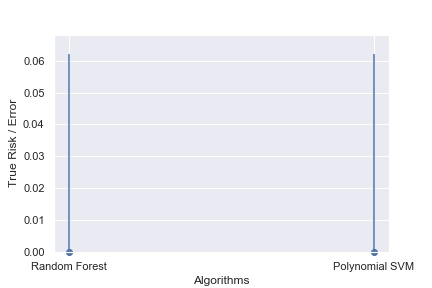
\includegraphics[scale=0.4]{img/binary_errorgraph1.jpg}
		\end{subfigure}
		\begin{subfigure}{0.4\textwidth}
			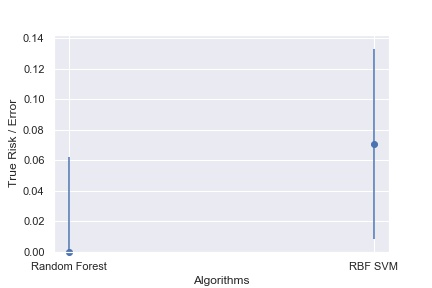
\includegraphics[scale=0.4]{img/binary_errorgraph2.jpg}
		\end{subfigure}
		\caption{\textbf{Left}: Confidence interval graph comparing Random Forest and SVM with polynomial kernel. \textbf{Right}: Confidence interval graph comparing Random Forest and SVM with RBF kernel.}
	\end{figure}
	\subsection{Classification with 3 Classes Comparison}
	From the results above for classification with 3 classes, the Random Forest had a 0.42\% loss versus SVM which had a 0.21\% loss (taking the polynomial kernel which had the least loss). The 95\% confidence interval for the true risk of Random Forest is [0, 0.0661] and for SVM is [0, 0.0641]. For classification with 3 classes, it is clear that SVM with polynomial kernel performs better as its upper bound of the 95\% confidence interval is slightly lower than the one for Random Forest but these 2 algorithms don't have significant difference in the true risk. A graph is shown below for these confidence interval:
	\begin{figure}[H]
		\centering
		\begin{subfigure}{0.4\textwidth}
			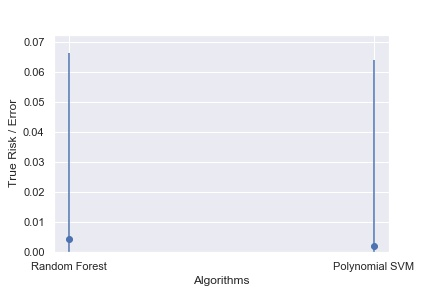
\includegraphics[scale=0.4]{img/3classes_errorgraph1.jpg}
		\end{subfigure}
		\begin{subfigure}{0.4\textwidth}
			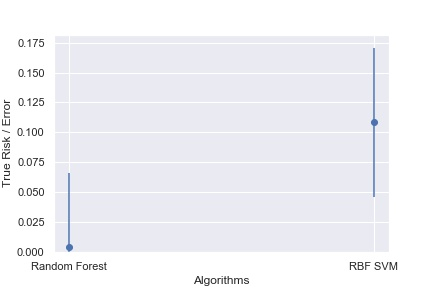
\includegraphics[scale=0.4]{img/3classes_errorgraph2.jpg}
		\end{subfigure}
		\caption{\textbf{Left}: Confidence interval graph comparing Random Forest and SVM with polynomial kernel. \textbf{Right}: Confidence interval graph comparing Random Forest and SVM with RBF kernel.}
	\end{figure}
	\noindent The figure above also shows that using RBF SVM leads to a more significant error increase when compared to Random Forest. In that case, Random Forest does have a lower upper bound making it the more safer algorithm to use. 
	 
	\subsection{Classification Using All Classes Comparison}
	The results above shows a significant difference in performance, the Random Forest had a 35.21\% loss versus the SVM which had a 42.08\% loss. The 95\% confidence interval for the risk will be [0.290, 0.414] and [0.359, 0.483] for Random Forest and SVM respectively. Compared to binary classification and classification with 3 classes, the loss has increased significantly, but just comparing these 2 confidence intervals, Random Forest performs better than SVM since both its upper bound and lower bound is lower than that of the SVM. A graph is presented below for better visualization. 
	\begin{figure}[H]
		\centering
		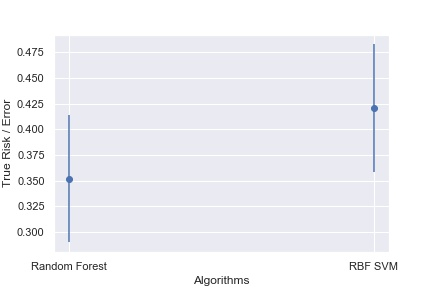
\includegraphics[scale=0.6]{img/allclasses_errorgraph1.jpg}
		\caption{ Confidence interval graph comparing Random Forest and SVM with RBF kernel.}
	\end{figure}
	
\end{document}